    \par\section{First Section}\label{sec:ch2.sec1}
    \par\subsection{Subsection A}\label{sec:ch2.sec1.subsec1}
    \par\noindent Lorem ipsum dolor sit amet, consectetur adipiscing elit. Maecenas lobortis dignissim turpis, a blandit neque molestie eget. Pellentesque maximus finibus est. Nulla gravida dolor at ante ultricies hendrerit. Nulla quis ornare magna, ac posuere dui.
    \par\noindent In eu nisl diam. Etiam vitae rutrum enim. Vestibulum id bibendum enim. Quisque dictum pretium nunc sed pretium. Interdum et malesuada fames ac ante ipsum primis in faucibus. Integer pulvinar ipsum quis nunc placerat, id rutrum magna ullamcorper.
    \par\noindent Sed nec felis vel mauris iaculis gravida. Aliquam orci massa, scelerisque eu risus ut, iaculis sollicitudin augue. Suspendisse faucibus pellentesque lacus, sed sodales leo maximus eget. Aliquam. 
    \par\noindent \autoref{fig:ch2.f1a} and \autoref{fig:ch2.f1b} in \autoref{fig:ch2.f1} are the demonstration of sub-figures.
    \par\begin{minipage}{\linewidth}
        \centering
        \begin{figure}[H]%
            \centering%
            \captionsetup[subfigure]{aboveskip=5pt,belowskip=5pt}%
            \centering%
            \begin{subfigure}[b]{0.45\textwidth}%
                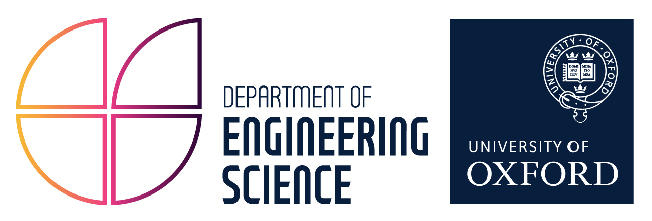
\includegraphics[width=\textwidth]{Images/CH2/EngLogo_PlaceHolder}%
                \subcaption{<Add the subcaption here if needed.>}%
                \label{fig:ch2.f1a}%
            \end{subfigure}%
            \hspace{40pt}%
            \begin{subfigure}[b]{0.45\textwidth}%
                
\includegraphics[width=\textwidth]{Images/CH2/SomervilleLogo_PlaceHolder}%
                \subcaption{}%
                \label{fig:ch2.f1b}%
            \end{subfigure}%
            \caption{(a) EngSci Logo (b) Somerville College Logo.}\label{fig:ch2.f1}%
        \end{figure}
    \end{minipage}%
    \par\noindent Lorem ipsum dolor sit amet, consectetur adipiscing elit. Donec rhoncus risus ex, scelerisque maximus nunc iaculis sit amet. Fusce vitae ipsum erat. Pellentesque habitant morbi tristique senectus et netus et malesuada fames ac turpis egestas.
    \par\subsection{Subsection B}\label{sec:ch2.sec1.subsec2}
    \par\noindent Lorem ipsum dolor sit amet, consectetur adipiscing elit. Etiam vitae leo aliquet, luctus sapien at, laoreet massa. Morbi eros lacus, elementum non tempus at, vestibulum ac enim. Curabitur tristique sagittis augue, quis molestie nisl ullamcorper quis. Etiam vel varius orci. Praesent nisi mauris, lacinia non lobortis at, viverra in purus. 
    \par\noindent \autoref{fig:ch2.f3} is the demonstration of a single figure.
    \par\begin{minipage}{\linewidth}
        \centering
        \begin{figure}[H]
            \centering    
            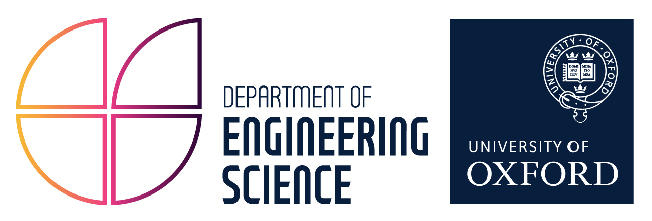
\includegraphics[width=0.55\linewidth]{Images/CH2/EngLogo_PlaceHolder}
            \caption{<Add the caption here.>}\label{fig:ch2.f3}
        \end{figure}
    \end{minipage}%
    \par\subsection{Subsection C}\label{sec:ch2.sec1.subsec3}
    Lorem ipsum dolor sit amet, consectetur adipiscing elit. Etiam vitae leo aliquet, luctus sapien at, laoreet massa. Morbi eros lacus, elementum non tempus at, vestibulum ac enim. 
    \par\noindent The equations with sub-index are demonstrated in \autoref{eq:ch2eq2}:
    \begin{subequations}
        \begin{align}
            f_{\text{elastic}}(\widehat{\mathbf{n}})&=f_{\text{splay}}(\widehat{\mathbf{n}})+f_{\text{twist}}(\widehat{\mathbf{n}})+f_{\text{bend}}(\widehat{\mathbf{n}})\\
            &=\frac{1}{2}\left\{K_{11}{\left[\nabla\cdot\widehat{\mathbf{n}}\right]}^{2}+K_{22}{\left[\widehat{\mathbf{n}}\cdot\nabla\times\widehat{\mathbf{n}}\right]}^{2}+K_{33}{\left[\widehat{\mathbf{n}}\times\nabla\times\widehat{\mathbf{n}}\right]}^{2}\right\}\label{eq:ch2eq2}
        \end{align}
    \end{subequations}
    Lorem ipsum dolor sit amet, consectetur adipiscing elit. Fusce feugiat viverra sodales. Fusce euismod dui vel leo placerat, ac mollis sem aliquet. 
    \par\noindent The simple equation with index is demonstrated in \autoref{eq:ch2eq3}:
    \begin{equation}
        f_{\text{elastic}}(\widehat{\mathbf{n}})=\frac{1}{2}K\left\{{\left[\nabla\cdot\widehat{\mathbf{n}}\right]}^{2}+{\left[\nabla\times\widehat{\mathbf{n}}\right]}^{2}\right\}\label{eq:ch2eq3}
    \end{equation}
    \par\subsection{Subsection D}\label{sec:ch2.sec1.subsec4}
    \par\subsubsection{Subsubsection I}\label{sec:ch2.sec1.subsec4.subsubsec1}
    \par\noindent Lorem ipsum dolor sit amet, consectetur adipiscing elit. Fusce feugiat viverra sodales. Fusce euismod dui vel leo placerat, ac mollis sem aliquet.  
    \par\noindent The array expression is demonstrated in \autoref{eq:ch2eq7}:
    \begin{singlespace}
        \begin{equation}
            \varepsilon_{r}=\left(
            \begin{array}{ccc}
                \varepsilon_{\perp}&0&0\\
                0&\varepsilon_{\perp}&0\\
                0&0&\varepsilon_{\parallel}
            \end{array}\right)\label{eq:ch2eq7}
        \end{equation}
    \end{singlespace}
    where $\varepsilon_{\perp}$ and $\varepsilon_{\parallel}$ are the examples of in-text equations.
    \par\subsubsection{Subsubsection II}\label{sec:ch2.sec1.subsec4.subsubsec2}
    \par\noindent Lorem ipsum dolor sit amet, consectetur adipiscing elit. Fusce feugiat viverra sodales. Fusce euismod dui vel leo placerat, ac mollis sem aliquet.
    \par\subsection{Subsection E}\label{sec:ch2.sec1.subsec5}
    \par\subsubsection{Subsubsection I}\label{sec:ch2.sec1.subsec5.subsubsec1}
    \par\noindent Lorem ipsum dolor sit amet, consectetur adipiscing elit. Fusce feugiat viverra sodales. Fusce euismod dui vel leo placerat, ac mollis sem aliquet.
    \par\subsubsection{Subsubsection II}\label{sec:ch2.sec1.subsec5.subsubsec2}
    \par\noindent Lorem ipsum dolor sit amet, consectetur adipiscing elit. Fusce feugiat viverra sodales. Fusce euismod dui vel leo placerat, ac mollis sem aliquet.
    \par\noindent \autoref{eq:ch2.eq21}, \autoref{eq:ch2.eq22}, \autoref{eq:ch2.eq23} demonstrate the chemical equations with individual indexes:
    \begin{gather}
        \ce{PI ->[hv + hv] PI^{*} -> R. + R.}\label{eq:ch2.eq21}\\
        \ce{R. + M -> RM. ->[\text{M}] RMM. {\cdots} -> RM_{n}.} \label{eq:ch2.eq22}\\
        \ce{RM_{n}. + RM_{m}. -> RM_{n + m}R}\label{eq:ch2.eq23}
    \end{gather}
    \par\noindent Some examples of crossref are shown as: \autoref{sec:ch2.sec1}, \autoref{sec:ch2.sec1.subsec1}, \autoref{sec:ch2.sec1.subsec2}, \autoref{sec:ch2.sec1.subsec3}, \autoref{sec:ch2.sec1.subsec4}, \autoref{sec:ch2.sec1.subsec5}, \autoref{sec:ch2.sec1.subsec4.subsubsec1}, \autoref{sec:ch2.sec1.subsec4.subsubsec2}, \autoref{sec:ch2.sec1.subsec5.subsubsec1}, \autoref{sec:ch2.sec1.subsec5.subsubsec2}.